% ============================================================================================
% record.tex -- project-level record: progress since Checkpoint 2, positioning, claim ledger,
% reproducibility practice, limitations. Fragment (no preamble). All figures under
% figures/record/, generated by scripts/record/{repo_history,make_figures,verify_record}.py.
% Repository state: commit 61d18d8 (2026-11-12). Old report: Checkpoint 2, compiled 2026-09-18.
% Each \subsection below is self-contained and may be moved independently.
% ============================================================================================

\section{The Project Record since Checkpoint~2}
\label{sec:record}

The Checkpoint~2 report was compiled when the repository stood at the merge of pull request~\#1
(commit \texttt{c9144e6}, 2026-09-18). At that point it held the original HTN model, the fixed-action-pattern (FAP)
and A* variants (neither of which that report mentions), and the configurable \texttt{spider\_\allowbreak{}web\_\allowbreak{}htn\_\allowbreak{}updated} package with its tests,
flat random-walker baseline and sensitivity sweeps. Since then the Python code has grown from 6,545 to
11,730 lines (excluding vendored code), the moving-support benchmark (versions 1--4) and a separate recovery
benchmark have been built, run and archived, and the team has adopted an explicit research record:
a dated work log, a binding claim ledger, curated evidence files with input hashes, and a
literature review that states what the biology does and does not license. This section gives the
chronology of that work and its positioning in the literature. The technical content of the new studies
follows in Sections~\ref{sec:core}--\ref{sec:sim}; the status of every claim, the reproducibility
practice and the limitations are collected afterwards in Section~\ref{sec:record-b}.

% --------------------------------------------------------------------------------------------
\subsection{Progress since Checkpoint~2}
\label{sec:record-progress}

\paragraph{Chronology.}
Table~\ref{tab:record-progress} combines the Git history (20 commits by three contributors) with
the repository's research work log (\texttt{docs/\allowbreak{}research/\allowbreak{}WORK\_\allowbreak{}LOG.md}). The two sources must be
read together: almost all of the moving-support and recovery work was done in working sessions
dated 2026-10-19 to 2026-10-24 on a branch \texttt{feat\_mulder} and committed in one commit on
2026-10-27, so the Git dates alone would hide the order in which the studies were built. The work log
itself warns that its dates ``identify session stages; exact execution timestamps were not
reconstructed retroactively''. Figure~\ref{fig:record-timeline} shows the commits, the milestones
and the growth of the code and test suite measured on every commit's tree.

{\small
\setlength{\tabcolsep}{4pt}
\begin{longtable}{@{}p{0.11\linewidth}p{0.15\linewidth}p{0.50\linewidth}p{0.17\linewidth}@{}}
\caption{Dated account of the work added after Checkpoint~2. ``Git'' rows are commits
(\texttt{git log --date=short}); ``log'' rows are entries of \texttt{docs/\allowbreak{}research/\allowbreak{}WORK\_\allowbreak{}LOG.md}.
Trial and test counts are those stated in the work log for that stage; the last row's test count was
re-run by us (Section~\ref{sec:record-repro}).}
\label{tab:record-progress}\\
\toprule
Date & Source & What was added or done & Scale \\
\midrule
\endfirsthead
\toprule
Date & Source & What was added or done & Scale \\
\midrule
\endhead
\bottomrule
\endfoot
2026-09-18 & Git \texttt{c9144e6} & State described by Checkpoint~2: \texttt{spider\_web\_htn}, \texttt{\_fap},
  \texttt{\_astar}, \texttt{\_htn\_updated} (configuration, stochasticity, baseline, sensitivity CSVs). &
  6,545 Python lines; 55 tests \\
2026-10-19 & log & Read Mulder et al.\ (2021)~\cite{mulder2021dynamic}; created \texttt{feat\_mulder}; uncommitted
  adaptive-planner work saved in a named Git stash, kept out of the new experiments. & -- \\
(undated) & log & Mulder \emph{v1}: \texttt{spider\_\allowbreak{}web\_\allowbreak{}mulder} with affine support shear and six execution
  policies; endpoint execution; pilot and 0.049 vs.\ 0.05\,Hz comparison. & 270 + 180 trials \\
2026-10-20 & log & Mulder \emph{v2}: controller audit (action/decision/repair ledgers, isolated
  first-failure replays), three controller corrections. & 180 trials; 98 tests \\
2026-10-20 & log & Mulder \emph{v3} paper-facing study: continuous tracking, sensory lag, flat-sequence
  ablation, \texttt{phase\_wait} method, rigid-only calibration import (no raw data). & 2,280 trials; 114 tests \\
2026-10-20 & log & Research record created (index, claim ledger, curated evidence, manuscript fragments,
  \texttt{AGENTS.md}); Bansod et al.\ review; planner-strategy audit. & toy probe \\
2026-10-20 & log & Recovery \emph{v1}: upstream IPyHOP vendored at \texttt{bdda210}; separate
  \texttt{spider\_\allowbreak{}web\_\allowbreak{}recovery} package with four back-ends and seven scenarios. & 2,240 trials; 158 tests \\
2026-10-20 & log & Mulder \emph{v4}: IPyHOP integrated into the actual Mulder HTN; three back-ends;
  whole-suffix GTPyhop control. & 2,160 + 10 trials; 176 tests \\
2026-10-20 & log & Objective re-centred: \texttt{MULDER\_\allowbreak{}OBJECTIVE\_\allowbreak{}ROADMAP.md} (milestones, publication
  assessment). & -- \\
2026-10-24 & log & Last software check before the backup (stated in the 2026-10-27 entry). & 176 tests passed \\
2026-10-27 & Git \texttt{20e7015} & Mulder, recovery, vendored IPyHOP, documentation and evidence committed;
  all 3,046 generated result files archived in \texttt{research\_\allowbreak{}snapshots/\allowbreak{}} with a per-file SHA-256 manifest. &
  10,629 Python lines; 176 tests \\
2026-11-12 & Git \texttt{7e59389} & \texttt{AGENTS.md} revised; \texttt{RESEARCH\_\allowbreak{}RECORD\_\allowbreak{}GUIDELINES.md} added. & -- \\
2026-11-12 & Git \texttt{d2e639b} & ``Data files for manuscript'': the 3,046 result files committed under
  \texttt{mulder\_results/} on \texttt{main}. & 3,046 files \\
2026-11-12 & Git \texttt{2b01e41} & \texttt{feat\_mulder} merged into \texttt{main}. & -- \\
2026-11-12 & Git \texttt{61d18d8}, log & Spider literature search (11 sources, 14 bibliography keys,
  experiments E1--E3 proposed only); adaptive-planner work restored from its stash
  (\texttt{instrumentation.py}, \texttt{perturbations.py}, \texttt{spiral\_\allowbreak{}geometry.py}, silk capacity,
  visualiser) with the historical \texttt{perturbation\_\allowbreak{}trials.csv}. & 11,730 Python lines; 177 tests \\
\end{longtable}
}

\begin{figure}[t]
  \centering
  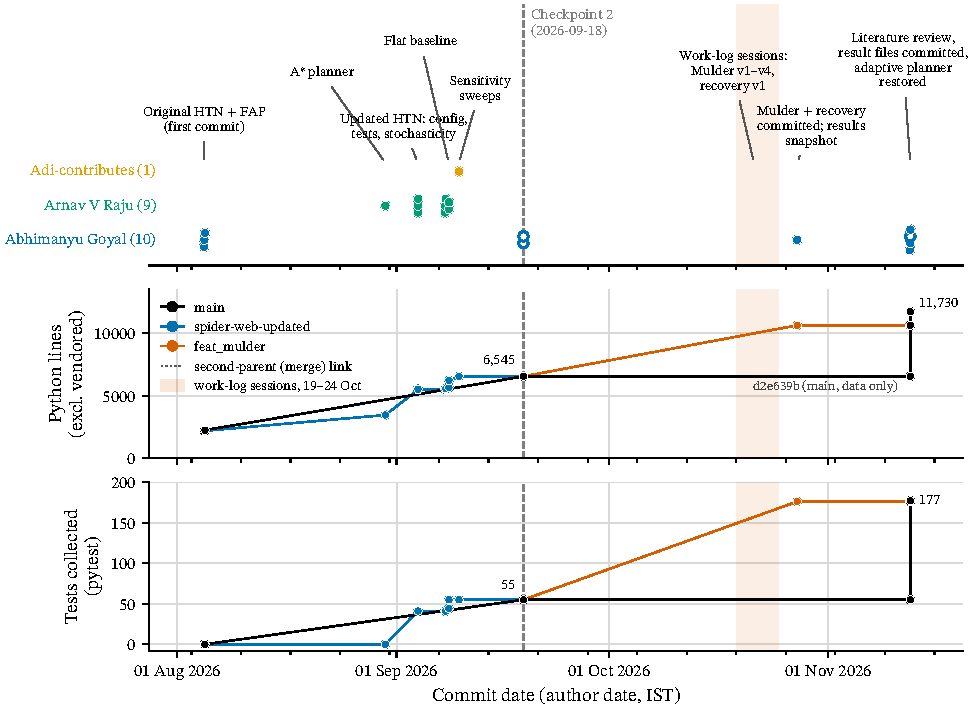
\includegraphics[width=\linewidth]{figures/record/record_timeline}
  \caption{Project timeline. \emph{Top:} all 20 commits, one lane per Git author (commit count in
  brackets; commits on the same day are stacked vertically; hollow markers are merge commits),
  with the main milestones. The dashed line marks Checkpoint~2 (\texttt{c9144e6}); the shaded band
  marks the work-log sessions of 19--24 October, which were committed only on 27 October.
  \emph{Middle and bottom:} Python lines (\texttt{wc -l}, all tracked \texttt{*.py} files including
  tests, excluding the vendored \texttt{third\_\allowbreak{}party/\allowbreak{}IPyHOP}) and pytest-collected tests, measured on
  each commit's own tree and drawn along the commit graph (solid: first parent; dotted: merged
  parent). The low point on 12 November is \texttt{d2e639b}, a data-only commit on \texttt{main}
  made before \texttt{feat\_mulder} was merged. $n=20$ commits. Data: \texttt{git log} of the
  repository at \texttt{61d18d8}, measured by \texttt{scripts/\allowbreak{}record/\allowbreak{}repo\_\allowbreak{}history.py}.}
  \label{fig:record-timeline}
\end{figure}

\paragraph{Repository structure.}
Table~\ref{tab:record-packages} lists every package at \texttt{61d18d8}. Line counts are
\texttt{wc -l} over the tracked Python files; test counts were obtained by running
\texttt{pytest --collect-only} per package on a private clone, and the full suite was then run
(177 passed; Section~\ref{sec:record-repro}). Only three packages have test suites; the original
HTN, FAP and A* packages have none, and all three are unchanged since Checkpoint~2
(\texttt{git diff c9144e6 61d18d8} is empty for them; Figure~\ref{fig:record-composition}). Besides Python, \texttt{visualization/} holds 7,703 lines of
HTML/JavaScript viewers and generated plan data (plus 481 lines under
\texttt{spider\_\allowbreak{}web\_\allowbreak{}astar/\allowbreak{}visualization/\allowbreak{}}), which are not counted in the table.

{\footnotesize
\setlength{\tabcolsep}{3.5pt}
\begin{longtable}{@{}p{0.24\linewidth}p{0.22\linewidth}r r r p{0.27\linewidth}@{}}
\caption{Repository packages at commit \texttt{61d18d8}. ``Src'' and ``Test'' are Python source and
test-file lines (\texttt{wc -l}); ``Tests'' is the number collected by pytest. A dagger marks packages
added after Checkpoint~2.}
\label{tab:record-packages}\\
\toprule
Package & Role & Src & Test & Tests & Where its results live \\
\midrule
\endfirsthead
\toprule
Package & Role & Src & Test & Tests & Where its results live \\
\midrule
\endhead
\bottomrule
\endfoot
\texttt{spider\_web\_htn} & Original Zschokke HTN (Checkpoint~2, Sections~1--6) & 1,279 & 0 & 0 &
  Printed plan; \texttt{visualization/\allowbreak{}index.html}, \texttt{plan\_data.js} \\
\texttt{spider\_web\_fap} & Fixed-action-pattern variant & 785 & 0 & 0 & Printed plan only (no committed outputs) \\
\texttt{spider\_\allowbreak{}web\_\allowbreak{}astar} & A* planner (superseded in \texttt{insights.md}) & 1,267 & 0 & 0 &
  \texttt{visualization/\allowbreak{}index\_\allowbreak{}astar.html}, \texttt{plan\_\allowbreak{}data\_\allowbreak{}astar.js}; \texttt{empirical\_\allowbreak{}data.md} \\
\texttt{spider\_\allowbreak{}web\_\allowbreak{}htn\_\allowbreak{}updated} & Configurable HTN, baseline, sweeps, perturbations, instrumentation & 3,317 & 827 & 56 &
  Root CSVs: \texttt{sensitivity\_\allowbreak{}comparison}, \texttt{wind\_\allowbreak{}sensitivity}, \texttt{single\_\allowbreak{}run\_\allowbreak{}comparison},
  \texttt{perturbation\_\allowbreak{}trials} (C28); \texttt{visualization/\allowbreak{}index\_\allowbreak{}updated.html} \\
\texttt{spider\_\allowbreak{}web\_\allowbreak{}mulder}$^\dagger$ & Moving-support benchmark, v1--v4 & 2,121 & 619 & 77 &
  \texttt{mulder\_\allowbreak{}results/\allowbreak{}\{pilot, frequency\_\allowbreak{}0049\_\allowbreak{}vs\_\allowbreak{}005, controller\_\allowbreak{}audit\_\allowbreak{}v2, paper\_\allowbreak{}validation\_\allowbreak{}v3*, mulder\_\allowbreak{}reentrant\_\allowbreak{}v4\}};
  \texttt{docs/\allowbreak{}research/\allowbreak{}evidence/\allowbreak{}mulder\_\allowbreak{}*.json}; \texttt{docs/\allowbreak{}manuscript/\allowbreak{}figures/\allowbreak{}} \\
\texttt{spider\_\allowbreak{}web\_\allowbreak{}recovery}$^\dagger$ & Retained-tree recovery benchmark, v1 & 785 & 178 & 44 &
  \texttt{mulder\_\allowbreak{}results/\allowbreak{}recovery\_\allowbreak{}v1\_\allowbreak{}verified}; \texttt{evidence/\allowbreak{}recovery\_\allowbreak{}v1\_\allowbreak{}summary.json}, \texttt{recovery\_\allowbreak{}example/\allowbreak{}} \\
\texttt{docs/\allowbreak{}research/\allowbreak{}probes}$^\dagger$ & Strategy audit, suffix control, evidence snapshot scripts & 381 & 0 & 0 &
  \texttt{docs/\allowbreak{}research/\allowbreak{}evidence/\allowbreak{}*.json} \\
\texttt{third\_\allowbreak{}party/\allowbreak{}IPyHOP}$^\dagger$ & Vendored upstream planner, unmodified & 1,097 & 0 & 0 & -- \\
Root scripts & \texttt{run.py}, \texttt{run\_fap.py}, \texttt{visualize.py} & 171 & 0 & 0 & -- \\
\midrule
Total (excl.\ vendored) & & 10,106 & 1,624 & 177 & \\
\end{longtable}
}

\begin{figure}[t]
  \centering
  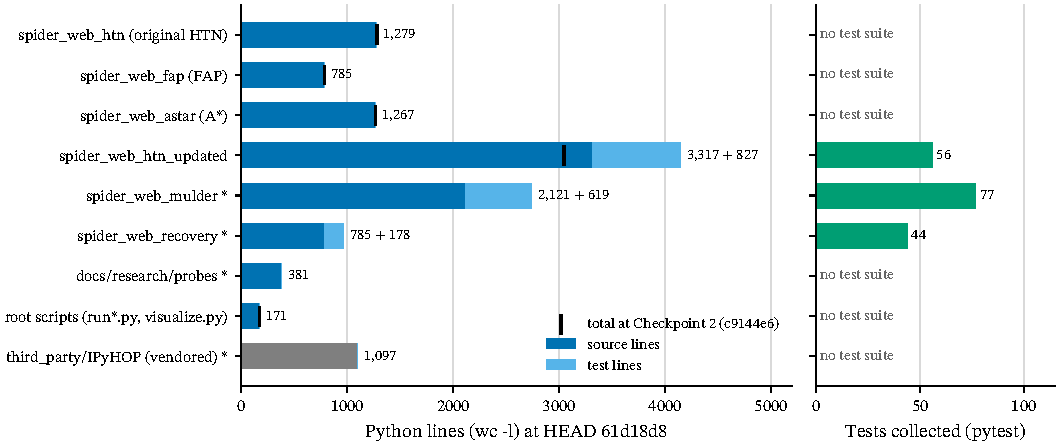
\includegraphics[width=\linewidth]{figures/record/record_composition}
  \caption{Repository composition at \texttt{61d18d8}. \emph{Left:} Python source lines (dark blue;
  grey for the vendored IPyHOP) and test-file lines (light blue) per package, with the package's total
  at Checkpoint~2 (\texttt{c9144e6}) marked by a black tick; an asterisk marks packages added after
  Checkpoint~2. \emph{Right:} tests collected by pytest per package (177 in total; all 177 passed when
  we re-ran them). Data: tracked files of the repository, measured by
  \texttt{scripts/\allowbreak{}record/\allowbreak{}repo\_\allowbreak{}history.py}.}
  \label{fig:record-composition}
\end{figure}

\paragraph{Roadmap status.}
Table~4 of the Checkpoint~2 report mapped the evaluation roadmap to files.
Table~\ref{tab:record-roadmap} updates it. Two points about its sources. First, the roadmap itself
(called ``Way-Forward'' and \texttt{future plan.pdf} in the module docstrings) is not in the repository;
the items below are taken from the docstrings that cite it. Second, \texttt{HTN Coding Plan.pdf}, which
\emph{is} in the repository, is a different and earlier document: a two-page implementation pipeline
(state, operators, opportunistic early-stage methods, stereotyped late-stage methods, distance-as-cost,
``GTPyhop's built-in backtracking'') that the original \texttt{spider\_web\_htn} package implements.
Its final point is now qualified by the planner-strategy audit (second row of the table and
Section~\ref{sec:record-repro}).

{\small
\setlength{\tabcolsep}{3.5pt}
\begin{longtable}{@{}p{0.23\linewidth}p{0.27\linewidth}p{0.44\linewidth}@{}}
\caption{Roadmap items, files and status, extending Table~4 of the Checkpoint~2 report. ``CP2'' = the
status given there; ``Now'' = status at \texttt{61d18d8} according to the repository record.}
\label{tab:record-roadmap}\\
\toprule
Item & File(s) & Status \\
\midrule
\endfirsthead
\toprule
Item & File(s) & Status \\
\midrule
\endhead
\bottomrule
\endfoot
\multicolumn{3}{@{}l}{\emph{Initial coding plan (\texttt{HTN Coding Plan.pdf})}}\\
State, operators, methods, distance-as-cost & \texttt{spider\_web\_htn/} & Implemented before Checkpoint~2
  (first commit, 2026-08-04). \\
``Built-in backtracking'' among proto-hub methods & \texttt{spider\_\allowbreak{}web\_\allowbreak{}htn/\allowbreak{}main.py} (\texttt{find\_plan}) &
  \emph{Now:} not established as measured behaviour. The installed GTPyhop~1.9.7 defaults to iterative greedy
  search with irrevocable commitment; the repository does not pin a strategy (C15, C22;
  \texttt{evidence/\allowbreak{}planner\_\allowbreak{}strategy\_\allowbreak{}audit.json}). \\
\midrule
\multicolumn{3}{@{}l}{\emph{Checkpoint~2 Table~4 items}}\\
Decouple domain/planner & \texttt{config.yaml}, \texttt{config\_\allowbreak{}loader.py} & CP2: implemented. Now: unchanged
  (\texttt{SPIDER\_\allowbreak{}WEB\_\allowbreak{}CONFIG} override). \\
Unit testing & \texttt{spider\_\allowbreak{}web\_\allowbreak{}htn\_\allowbreak{}updated/\allowbreak{}tests/\allowbreak{}} & CP2: 5 files, 55 tests. Now: 5 files, 56 tests
  (a regression test for the spiral operator's resource bound was added on 2026-11-12); plus 77 Mulder and
  44 recovery tests; 177 pass. \\
Data-driven parameterisation & \texttt{config.yaml} (\texttt{empirical:}) & CP2: implemented. Now: unchanged;
  not independently audited (\texttt{docs/\allowbreak{}research/\allowbreak{}README.md}). \\
Sensitivity analysis & \texttt{sensitivity.py} & CP2: ``wind currently off''. Now: the committed
  \texttt{wind\_\allowbreak{}sensitivity.csv} (9 wind levels, $2\times1{,}000$ trials each) and an anchor-removal sweep to
  $p=0.8$ already existed at \texttt{39b89f3} (2026-09-09); see the HTN-model section. \\
Comparison (Group A vs.\ B) & \texttt{baseline.py}, \texttt{compare.py} & Unchanged; the cross-package conclusion
  is not established (C17). \\
Replicability / seeding & \texttt{stochastic.py} & Unchanged (one seeded \texttt{random.Random} per run). \\
\midrule
\multicolumn{3}{@{}l}{\emph{Further roadmap items, restored 2026-11-12}}\\
Decomposition depth $D$ & \texttt{instrumentation.py} & Implemented (counts method-application attempts); not
  independently audited. \\
Perturbation trials and adaptation time $T_a$ & \texttt{perturbations.py}, \texttt{perturbation\_\allowbreak{}trials.csv} &
  Implemented. Recovered CSV is historical and unaudited (C28); only a one-seed smoke check was re-run. \\
Silk-capacity bound & \texttt{state.py}, \texttt{operators.py} (\texttt{\_has\_capacity}) & Implemented;
  unbounded by default, 2,200\,cm in the perturbation trials (cut by 30\% in the depletion stressor). \\
Spiral geometry, updated visualiser & \texttt{spiral\_\allowbreak{}geometry.py}, \texttt{visualize\_\allowbreak{}updated.py} & Implemented. \\
Pruning heuristic ($E_{\mathrm{total}}$ vs.\ $E_{\mathrm{capture}}$) & -- & Not implemented (left as future work in
  Checkpoint~2 Section~9; no code in the repository). \\
\midrule
\multicolumn{3}{@{}l}{\emph{Added beyond the roadmap}}\\
Moving-support benchmark & \texttt{spider\_\allowbreak{}web\_\allowbreak{}mulder/\allowbreak{}} & v1--v3 done; 2,280-trial v3 study (C01--C12). \\
Planner-strategy audit & \texttt{docs/\allowbreak{}research/\allowbreak{}probes/\allowbreak{}planner\_\allowbreak{}strategy.py} & Done (C15, C22). \\
Retained-tree recovery & \texttt{spider\_\allowbreak{}web\_\allowbreak{}recovery/\allowbreak{}}, \texttt{third\_\allowbreak{}party/\allowbreak{}IPyHOP/\allowbreak{}} & Done; 2,240 trials
  (C16, C18--C23). \\
IPyHOP inside the Mulder HTN & \texttt{reentrant.py}, \texttt{recovery\_\allowbreak{}comparison.py} & Done; 2,160 trials and a
  10-trial control (C24--C27). \\
Research record & \texttt{docs/research/}, \texttt{research\_\allowbreak{}snapshots/\allowbreak{}}, \texttt{AGENTS.md},
  \texttt{RESEARCH\_\allowbreak{}RECORD\_\allowbreak{}GUIDELINES.md} & Done; maintained since 2026-10-20. \\
Literature review & \texttt{SPIDER\_\allowbreak{}HTN\_\allowbreak{}LITERATURE.md}, \texttt{references.bib} & Done (2026-11-12);
  experiments E1--E3 proposed, not implemented. \\
\end{longtable}
}

% --------------------------------------------------------------------------------------------
\subsection{Related Work and Positioning}
\label{sec:record-related}

The repository's targeted literature search (\texttt{docs/\allowbreak{}research/\allowbreak{}SPIDER\_\allowbreak{}HTN\_\allowbreak{}LITERATURE.md},
2026-11-12) screened eleven sources. It is explicitly ``not a systematic review'', and several sources were
read only at abstract or metadata level; we report its conclusions, not a new survey.

\paragraph{Orb-web construction behaviour.}
Zschokke~\cite{zschokke1996early}, the basis of our original model, reports that early construction in
\emph{Araneus diadematus} draws on recurring but variable behavioural patterns, that behaviour becomes more
stereotyped after the proto-hub is established, and that reusing an existing framework costs less travel than
building at a new site. Peters~\cite{peters1970configuration} altered building sequences and transferred
spiders to partial webs, showing that the existing thread configuration affects subsequent construction and
can cause phases to be repeated. Eberhard~\cite{eberhard2019flexibility} documents flexibility in the cues
that guide construction in \emph{Zosis geniculata} and \emph{Uloborus diversus}, including temporary
exceptions that give access to parts of the web. Vollrath, Downes and Krackow~\cite{vollrath1997variability}
report geometry changes associated with support geometry, wind, temperature, humidity and silk supply.
Corver et al.~\cite{corver2021stages} describe stage-specific action sequences in \emph{U.~diversus} with a
hierarchical hidden Markov model, including atypical stage progressions. Mulder et
al.~\cite{mulder2021dynamic} compared construction on moving and stationary supports and reported that
dynamic environments do not appear to constrain web building; this paper is the reference for our
moving-support benchmark.

\paragraph{Rule-based and simulation models of web building.}
Artificial-intelligence modelling of web construction is established prior work. Gotts and
Vollrath~\cite{gotts1991modelling} initialised temporary-spiral models from reconstructed partial webs with
progressively simpler rules; Krink and Vollrath fitted construction-rule parameters with genetic algorithms
and compared artificial with laboratory webs~\cite{krink1997analysing}, and showed that matching auxiliary
and capture-spiral pitch can emerge from local interactions with existing threads~\cite{krink1998emergent};
Vollrath and Krink~\cite{vollrath2020robotics} discuss virtual spiders, local sensing and the morphological
contribution to feedback. Two consequences follow for our work: realistic final geometry does not by itself
show an advantage for a planner or reveal the animal's internal representation, and any claim of advantage
needs an equally informed rule-based comparison.

\paragraph{HTN planning and re-entrant planning.}
All our HTN models use GTPyhop (\url{https://github.com/dananau/GTPyhop}), now pinned at version 1.9.7.
The recovery studies use IPyHOP, the re-entrant HTN planner of Bansod, Nau, Patra and
Roberts~\cite{bansod2021reentrant}, which retains the solution task network, re-enters it at the failed node
from the newly observed state, removes later refinements conservatively (\textsc{Un-Refine-Post}) and lets the
actor execute only newly marked primitive tasks (\textsc{Run-Lazy-Refineahead}); a related paper treats
replanning ``from the middle''~\cite{bansod2022middle}. The repository's review
(\texttt{BANSOD\_\allowbreak{}REENTRANT\_\allowbreak{}REVIEW.md}) distinguishes three meanings of ``going back'' that the
Checkpoint~2 report did not separate: \emph{search backtracking} (abandoning a hypothetical refinement during
planning, with no physical motion), \emph{execution recovery} (revising unfinished work after a real failure,
with time, travel and position retained) and \emph{physical retracing} (moving back along existing threads,
which needs explicit traversal actions). Retained-tree recovery and selective replanning are prior work; we
integrate the unmodified upstream IPyHOP with a custom immediate-precondition actor and do not reproduce the
published Run-Lazy-Refineahead evaluation (C23).

\paragraph{Other domains.}
Cross and Jackson~\cite{cross2016detours} study planned detours in spider-eating jumping spiders and Hung,
Corver and Gordus~\cite{hung2026feedback} vibration-driven predator--prey feedback in an orb weaver. The
literature file recommends them only as optional discussion: neither concerns orb construction, and our graph
routes are not a replication of detour behaviour.

\paragraph{What the literature does and does not license.}
The literature file and the ledger (interpretation note of 2026-11-12) draw these conclusions:
\begin{itemize}
  \item It supports discussing behavioural stages, cue-dependent construction and existing rule-based models.
  \item It does \emph{not} establish HTN cognition in spiders, algorithmic novelty, or an HTN performance
    advantage. All HTN mappings are the team's proposed interpretations, not claims of the biological papers.
  \item Corver et al.'s hierarchical hidden Markov model is not an HTN; behavioural stages, HHMMs and
    hierarchical planning are different concepts.
  \item Searches for spiders with ``hierarchical task network'' or ``HTN planning'' found no verified
    biological HTN application in the screened results. This is not proof that none exists and does not
    justify a first-ever claim.
  \item No biological parameters, sample sizes or effect sizes were imported into any model from this search.
  \item The sensory-lag values used in our benchmark must not be attributed to Vollrath and
    Krink~\cite{vollrath2020robotics}, and wind is not equivalent to the moving-support shear.
\end{itemize}
Table~\ref{tab:record-literature} summarises, per source, the finding the file records, the HTN connection it
proposes and the caveat attached to it.

{\small
\setlength{\tabcolsep}{3pt}
\begin{longtable}{@{}p{0.15\linewidth}p{0.25\linewidth}p{0.22\linewidth}p{0.32\linewidth}@{}}
\caption{Literature used for positioning, as recorded in \texttt{docs/\allowbreak{}research/\allowbreak{}SPIDER\_\allowbreak{}HTN\_\allowbreak{}LITERATURE.md}.
``Access'' is the depth at which the file says the source was checked. All HTN connections are proposals,
not results; E1--E3 are the file's proposed (unimplemented) experiments.}
\label{tab:record-literature}\\
\toprule
Source (access) & Reported finding & Proposed HTN connection & Caveat recorded in the file \\
\midrule
\endfirsthead
\toprule
Source (access) & Reported finding & Proposed HTN connection & Caveat recorded in the file \\
\midrule
\endhead
\bottomrule
\endfoot
Zschokke 1996~\cite{zschokke1996early} (abstract, local PDF) & Variable early construction; more stereotyped
  after proto-hub; reuse of framework reduces travel & Alternative early methods; staged construction; new-site
  vs.\ reuse test & Initialising an existing scaffold is not evidence that the spider discovered or reused it \\
Peters 1970~\cite{peters1970configuration} (abstract) & Thread configuration affects construction; phase
  repetition after transfer to partial webs & Observed-state preconditions instead of completed-action history
  (E1) & Clearing a completion flag is not a transfer experiment \\
Eberhard 2019~\cite{eberhard2019flexibility} (author copy) & Flexible cue use; temporary exceptions &
  Alternative methods whose applicability depends on available structure (E1) & An expressive local rule can
  also implement exceptions; cognitive reading is the author's argument \\
Corver et al.\ 2021~\cite{corver2021stages} (full text, selected sections) & HHMM of stage-specific action
  sequences, atypical progressions & Reusable subtasks with conditional stage repetition (E2) & Not HTN evidence;
  data archive not downloaded; cross-species results kept separate \\
Vollrath et al.\ 1997~\cite{vollrath1997variability} (abstract) & Geometry varies with supports, weather, silk &
  Resource- and support-dependent methods (E3) & A model extension, not a parameter sweep \\
Gotts \& Vollrath 1991~\cite{gotts1991modelling} (abstract) & AI model initialised from real partial webs &
  HTN phase method vs.\ local rule on the same observations & Our flat execution is not a reproduction \\
Krink \& Vollrath 1997~\cite{krink1997analysing} (abstract, text) & GA-fitted rule parameters vs.\ laboratory
  webs & Equal-information rule vs.\ HTN with shared fitting budget & Geometry must be an output, not imposed \\
Krink \& Vollrath 1998~\cite{krink1998emergent} (abstract) & Spiral pitch emerges from local interactions &
  HTN chooses subtasks, local rules choose sites (E3) & Prescribed waypoints cannot test this honestly \\
Vollrath \& Krink 2020~\cite{vollrath2020robotics} (abstract, PDF) & Virtual spiders, local sensing, embodied
  feedback & Separate task selection from physical execution & Our lag values are not from this paper \\
Cross \& Jackson 2016~\cite{cross2016detours} (abstract, apparatus) & Planned detours in jumping spiders &
  Hierarchical navigation subtasks & Different behaviour; optional only \\
Hung et al.\ 2026~\cite{hung2026feedback} (abstract) & Vibration-guided predator--prey feedback & Future
  construction--sensing--capture integration & No predation model exists; optional only \\
\end{longtable}
}

\paragraph{Positioning.}
Following \texttt{MULDER\_\allowbreak{}OBJECTIVE\_\allowbreak{}ROADMAP.md} and the project memory (target journal: \emph{Programming and
Computer Software}), the contribution we can defend is a computational modelling and benchmark study with
informative negative results and reproducibility infrastructure. It is not a biological-verification study
(the original cohort data have not been obtained or fitted) and not a new planning algorithm (IPyHOP is
existing work). The roadmap names the strongest current question as \emph{when local feedback is sufficient
for moving-support construction and when broader replanning becomes useful}.
